
\DIFaddbegin 

\clearpage
\subsection{\DIFadd{The Wood merchant}}
\label{sec:appendix:moj:wood}

\DIFadd{A Viking carpenter was called a smithr. The waste wooden cores left over from making the cups are popular among children because they can use them as spinning tops.
}

\begin{display}{The wood stall}
	\label{fig:appendix:moj:places:wood:stall}
	\DIFadd{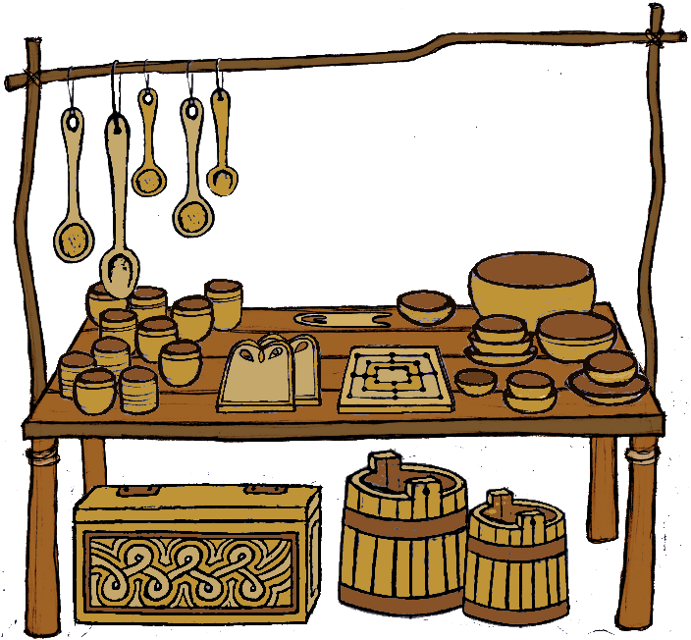
\includegraphics[width=0.65\columnwidth]{img/Jorvik/places/wood stall}
}\end{display}

\begin{display}{The wood stall with a background and a merchant}
	\label{fig:appendix:moj:places:wood}
	\DIFadd{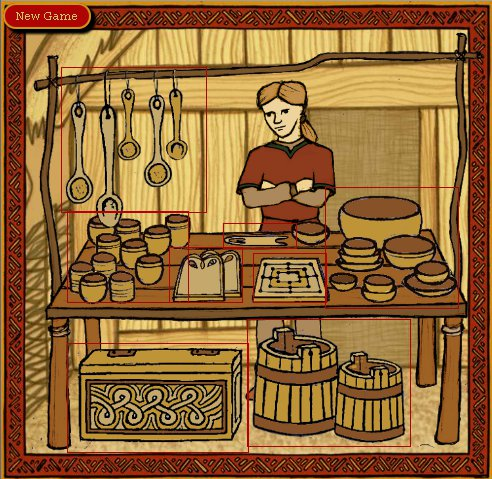
\includegraphics[width=0.65\columnwidth]{img/Jorvik/places/wood}
}\end{display}
\clearpage


\begin{table}[ht!]
	\centering
	\begin{tabular}{ p{3cm} c }\toprule
		\textbf{\DIFaddFL{Name:}} & \multirow{5}{*}{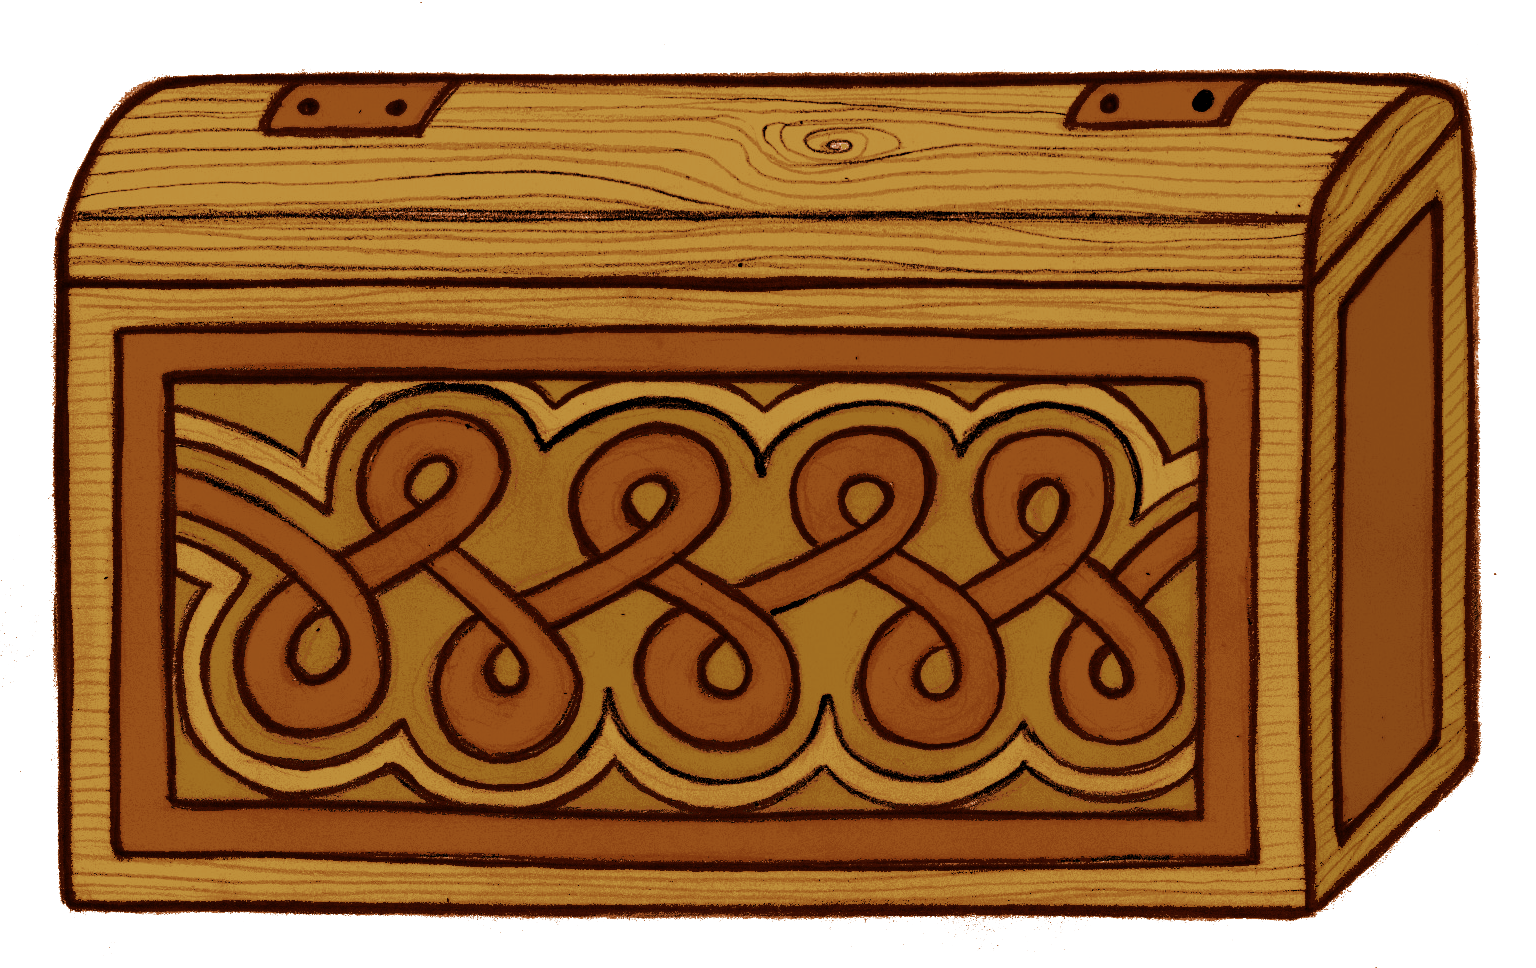
\includegraphics[height=30mm]{img/Jorvik/objects/wood/chest}}\\
		\DIFaddFL{Chest }& \\ 
		\textbf{\DIFaddFL{Price:}} & \\
		\DIFaddFL{35.29 silver. }& \\ 
		\textbf{\DIFaddFL{Description:}} & \\
		\multicolumn{2}{p{12cm}}{Most Viking homes had a wooden chest which the family would keep all of their valuable possessions locked inside.}\\
		\bottomrule
	\end{tabular}
\end{table}

\begin{table}[ht!]
	\centering
	\begin{tabular}{ p{3cm} c }\toprule
		\textbf{\DIFaddFL{Name:}} & \multirow{5}{*}{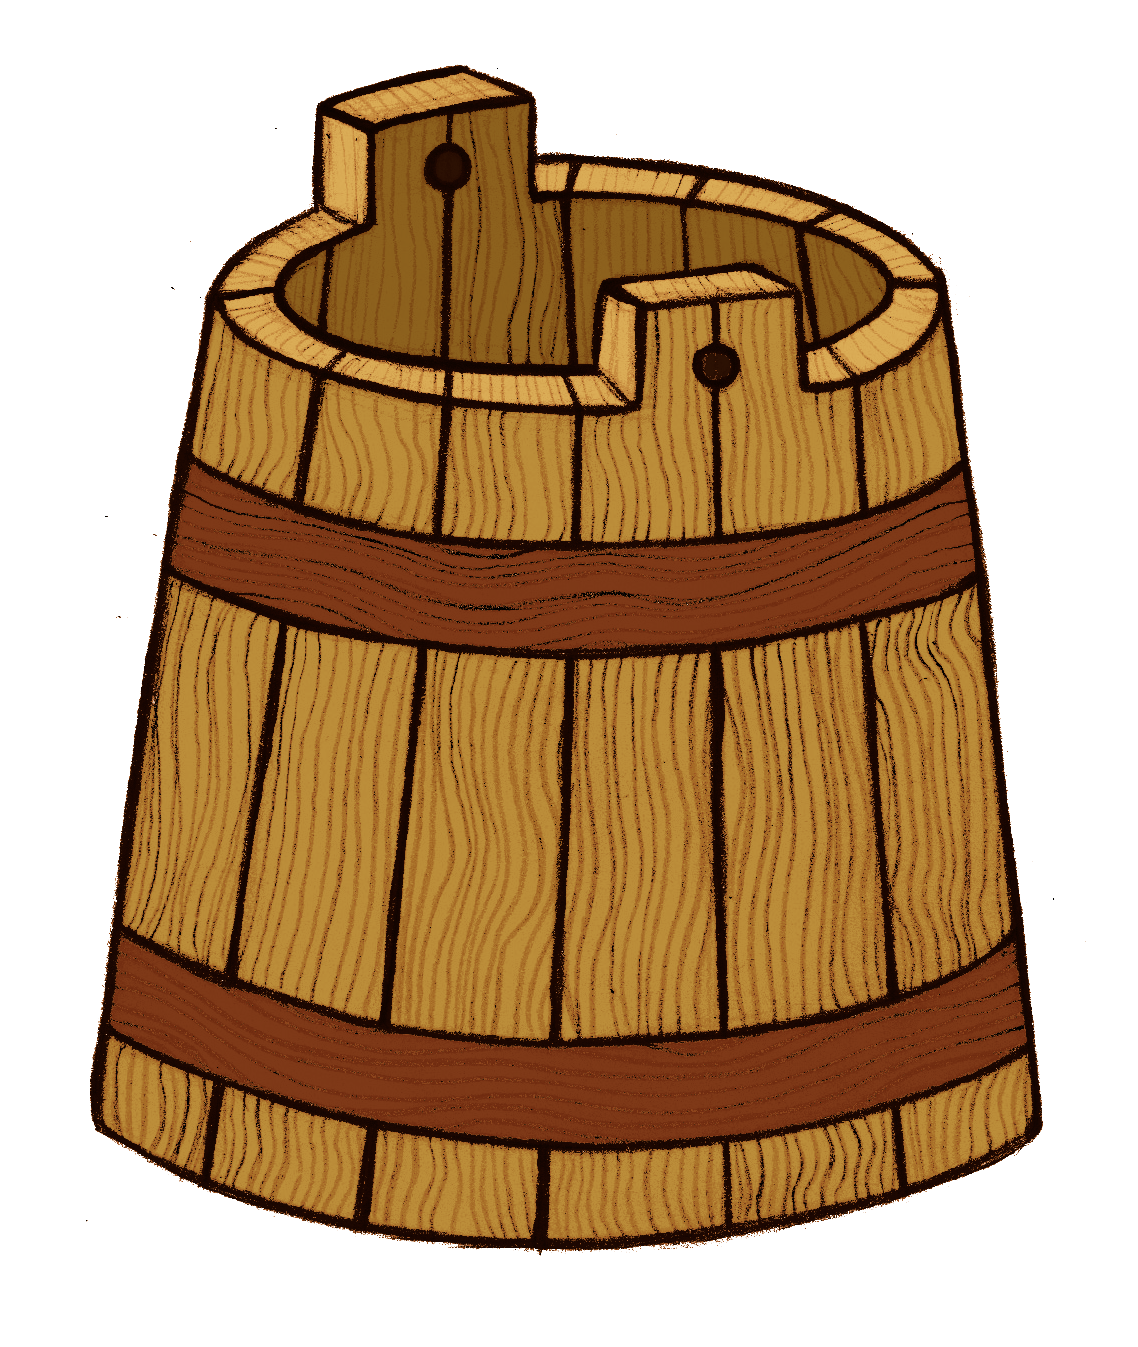
\includegraphics[height=30mm]{img/Jorvik/objects/wood/bucket}}\\
		\DIFaddFL{Bucket }& \\ 
		\textbf{\DIFaddFL{Price:}} & \\
		\DIFaddFL{17.64 silver. }& \\ 
		\textbf{\DIFaddFL{Description:}} & \\
		\multicolumn{2}{p{12cm}}{Buckets would have been made out of planks of wood and bound with metal hoops. Barrels and tubs were also made in this way.}\\
		\bottomrule
	\end{tabular}
\end{table}

\begin{table}[ht!]
	\centering
	\begin{tabular}{ p{3cm} c }\toprule
		\textbf{\DIFaddFL{Name:}} & \multirow{5}{*}{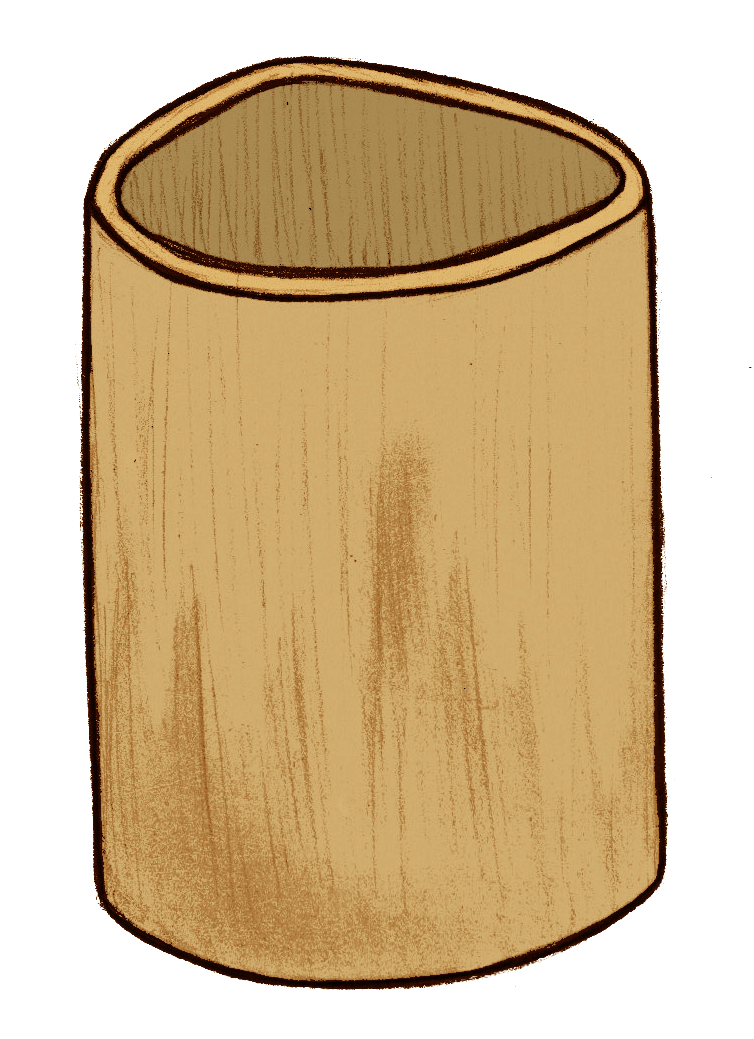
\includegraphics[height=30mm]{img/Jorvik/objects/wood/cup}}\\
		\DIFaddFL{Cup }& \\ 
		\textbf{\DIFaddFL{Price:}} & \\
		\DIFaddFL{0.44 silver. }& \\ 
		\textbf{\DIFaddFL{Description:}} & \\
		\multicolumn{2}{p{12cm}}{A pole lathe was a contraption that was powered by way of a treadle and used to make cups. The best wood for making cups was ash, alder and maple because they would not crack like oak.}\\
		\bottomrule
	\end{tabular}
\end{table}

\begin{table}[ht!]
	\centering
	\begin{tabular}{ p{3cm} c }\toprule
		\textbf{\DIFaddFL{Name:}} & \multirow{5}{*}{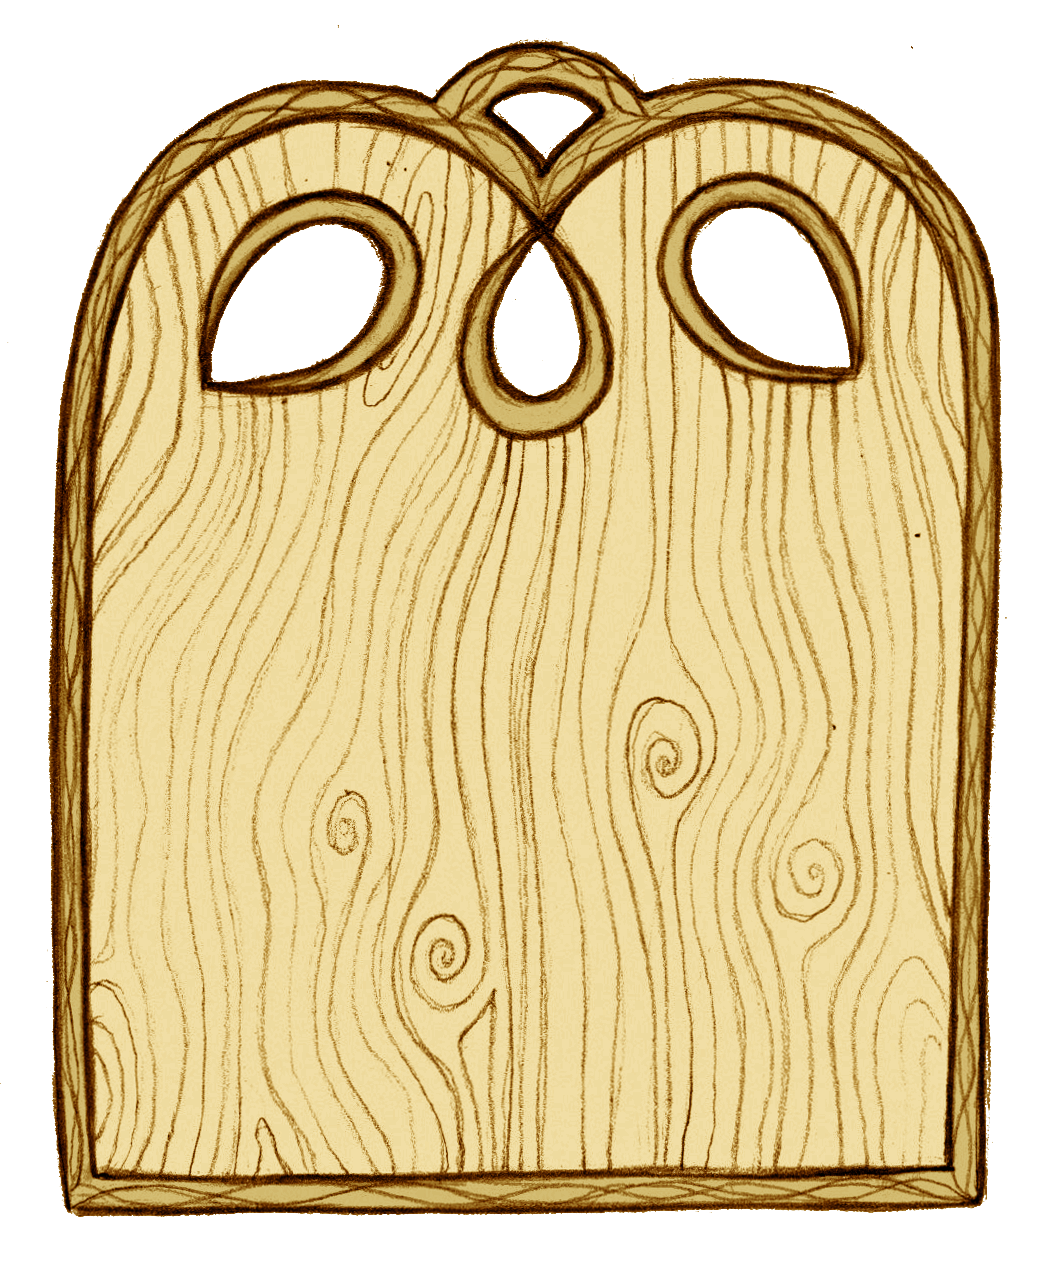
\includegraphics[height=30mm]{img/Jorvik/objects/wood/ironing board}}\\
		\DIFaddFL{Ironing Board }& \\ 
		\textbf{\DIFaddFL{Price:}} & \\
		\DIFaddFL{1.32 silver. }& \\ 
		\textbf{\DIFaddFL{Description:}} & \\
		\multicolumn{2}{p{12cm}}{Clothes would be ironed by rubbing a smooth, slick stone over them against a wooden or whalebone smoothing board whilst they were still wet. A method not too different from ironing today!}\\
		\bottomrule
	\end{tabular}
\end{table}

\begin{table}[ht!]
	\centering
	\begin{tabular}{ p{3cm} c }\toprule
		\textbf{\DIFaddFL{Name:}} & \multirow{5}{*}{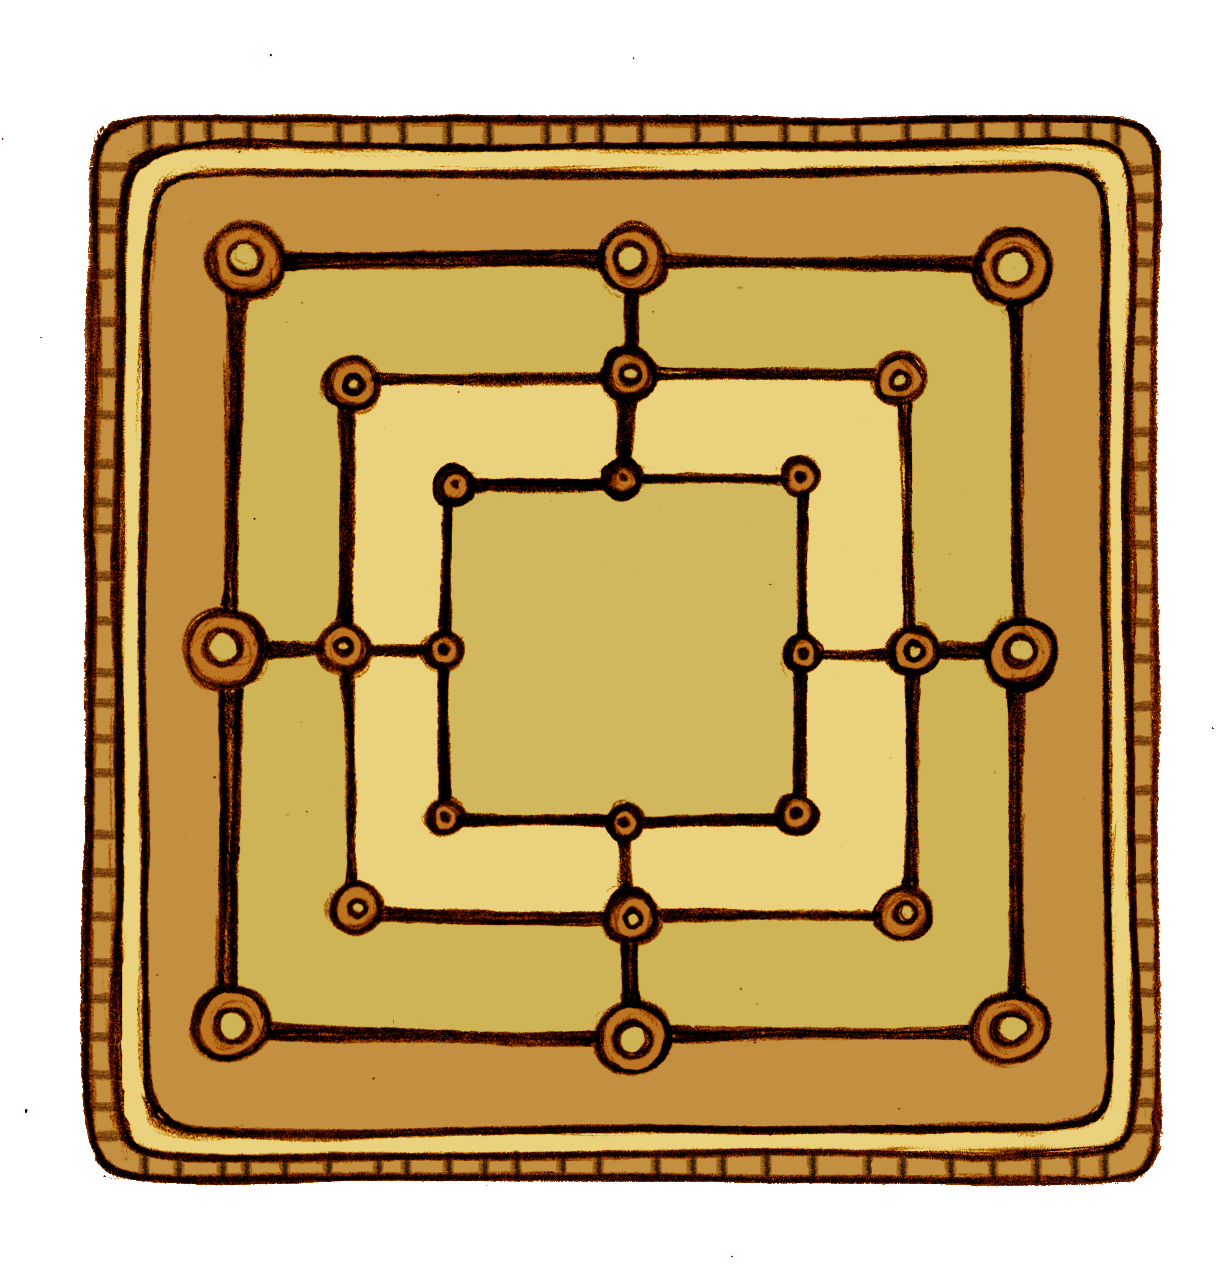
\includegraphics[height=30mm]{img/Jorvik/objects/wood/game board}}\\
		\DIFaddFL{Game Board }& \\ 
		\textbf{\DIFaddFL{Price:}} & \\
		\DIFaddFL{2.20 silver. }& \\ 
		\textbf{\DIFaddFL{Description:}} & \\
		\multicolumn{2}{p{12cm}}{Viking games like hnefatafl were played a lot to pass the time at home. Not only were they entertaining but they also taught children strategy and logic skills.}\\
		\bottomrule
	\end{tabular}
\end{table}

\begin{table}[ht!]
	\centering
	\begin{tabular}{ p{3cm} c }\toprule
		\textbf{\DIFaddFL{Name:}} & \multirow{5}{*}{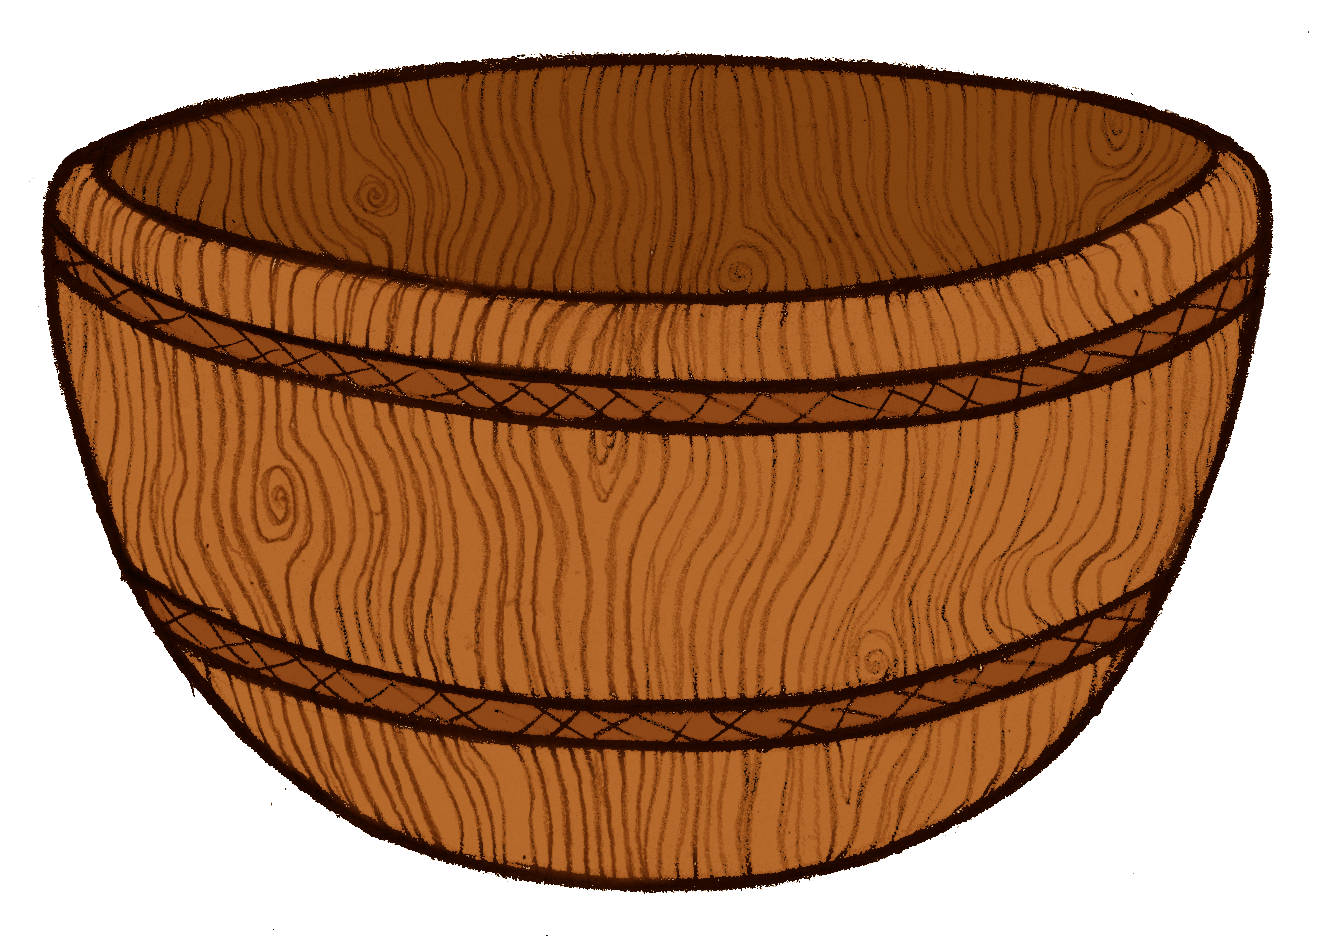
\includegraphics[height=30mm]{img/Jorvik/objects/wood/bowl}}\\
		\DIFaddFL{Bowl }& \\ 
		\textbf{\DIFaddFL{Price:}} & \\
		\DIFaddFL{0.44 silver. }& \\ 
		\textbf{\DIFaddFL{Description:}} & \\
		\multicolumn{2}{p{12cm}}{Bowls were made from wood and sometimes clay. Well-preserved Viking bowls could easily be mistaken for being modern.}\\
		\bottomrule
	\end{tabular}
\end{table}

\begin{table}[ht!]
	\centering
	\begin{tabular}{ p{3cm} c }\toprule
		\textbf{\DIFaddFL{Name:}} & \multirow{5}{*}{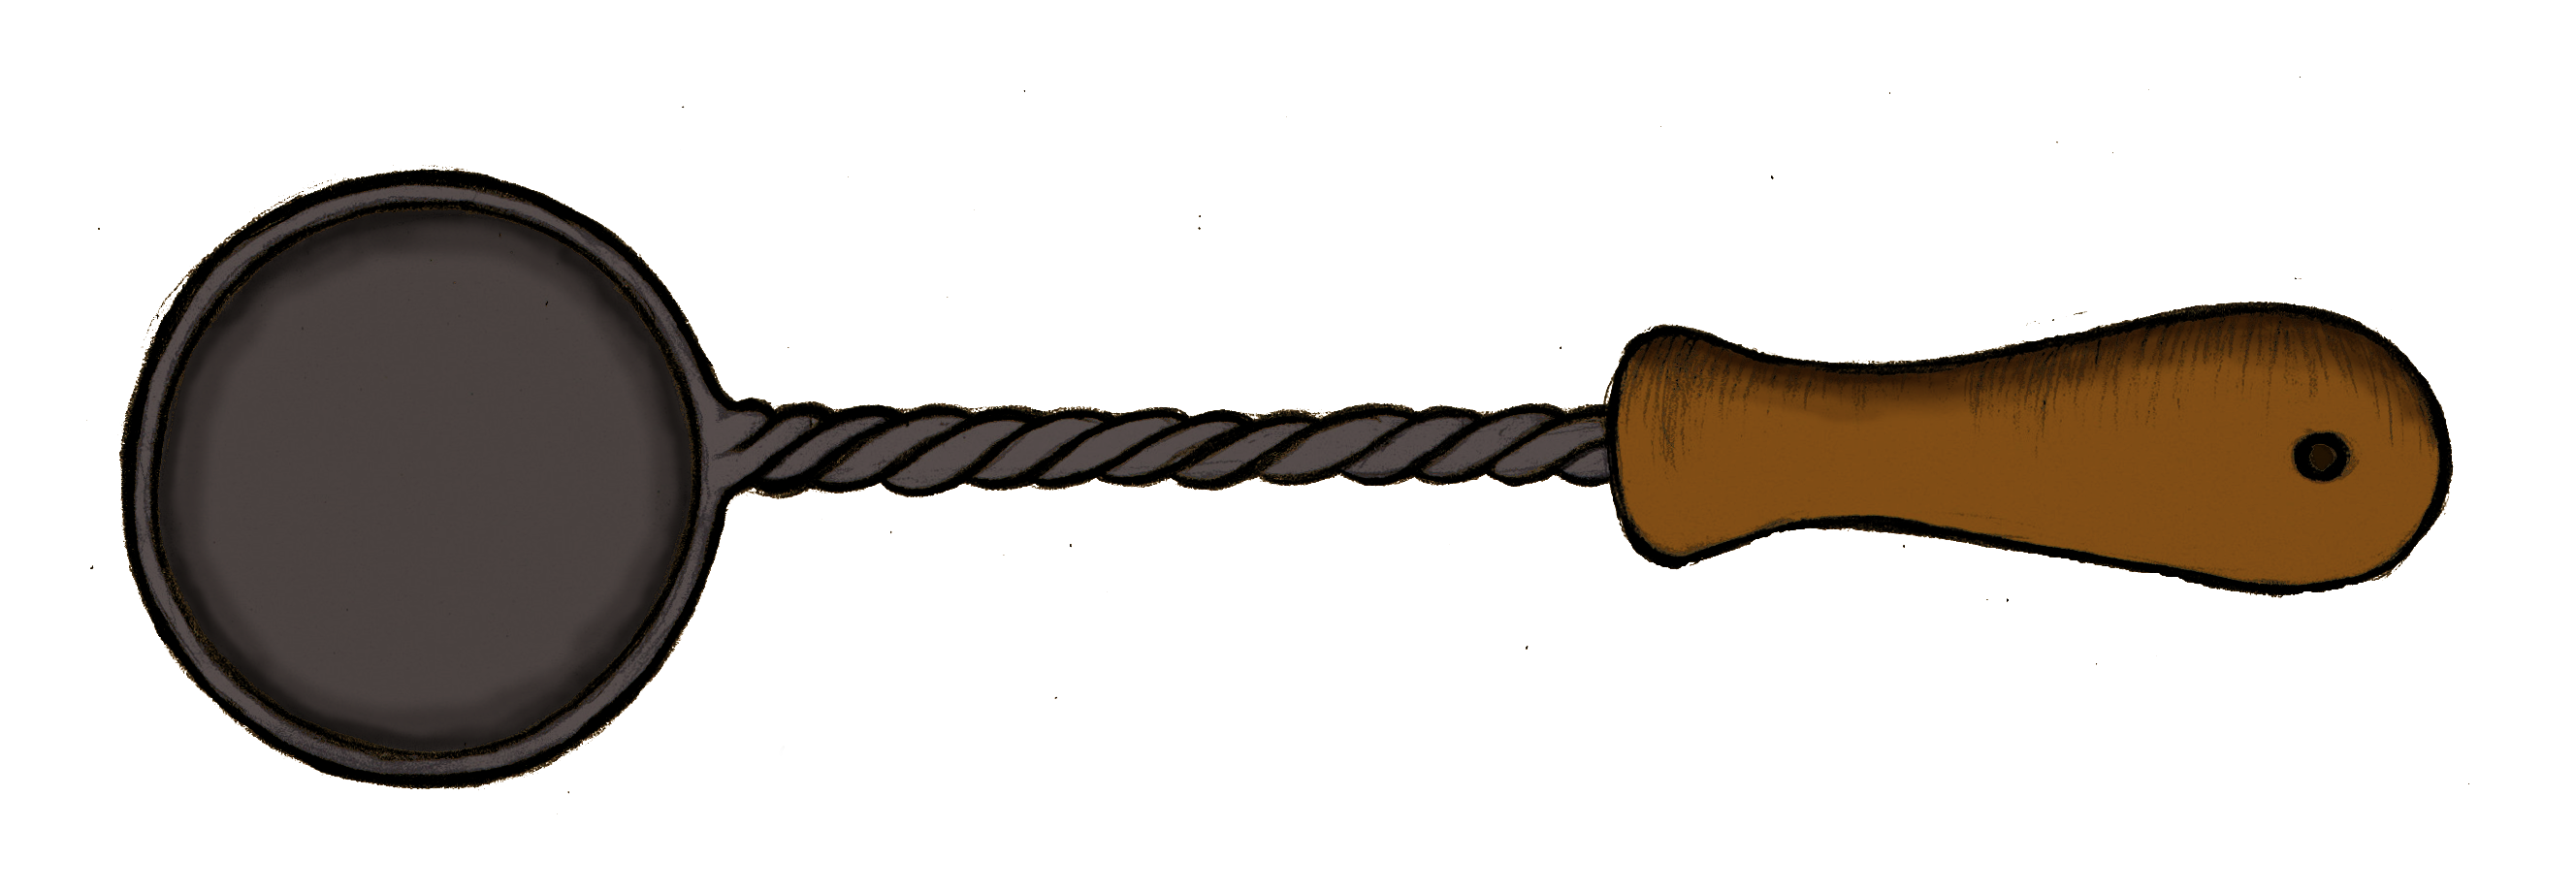
\includegraphics[width=70mm]{img/Jorvik/objects/wood/ladle}}\\
		\DIFaddFL{Ladle }& \\ 
		\textbf{\DIFaddFL{Price:}} & \\
		\DIFaddFL{0.88 silver. }& \\ 
		\textbf{\DIFaddFL{Description:}} & \\
		\multicolumn{2}{p{12cm}}{Ladles were used to serve drinks into cups for everyday use and drinking horns for cold alcoholic drinks at feasts. A Viking woman was found buried with a ladle and a bucket in Skei, Norway.}\\
		\bottomrule
	\end{tabular}
\end{table} \DIFaddend